\documentclass[german,version-2020-11]{uzl-thesis}
% !TeX program = lualatex

\UzLThesisSetup{
  Logo-Dateiname        = {institutslogo.pdf},
  Verfasst              = {am}{Institut für Informationssysteme},
  Titel auf Deutsch = { Evaluation eines Algorithmus zur Absicherung von Datenbanken mit Propabilistischen  },
  Titel auf Englisch = { Evaluation of an Algorithm for Securing Databases from Propabilsitic Inference},
  Autor                 = {Kevin Schmelzer},
  Betreuerin            = {Prof. Dr. Ralf Möller},
  Mit Unterstützung von = {Simon Schiff},
  Bachelorarbeit,
  Studiengang           = {IT-Sicherheit},
  Datum                 = {18. August 2020},
  Abstract              = {
   Englische Abstract
  },
  Zusammenfassung       = {
  	Datenbanken mit sensiblen Daten sollten einen hohen Sicherheitsstandard erfüllen. Trotzdem ist das einrichten von Sicherheitsvorkehrungen komplex und erfordert spezielle Fachkräfte, die sich mit den Systemen auskennen müssen. Diese Problematik haben viele Forschungseinrichtungen und auch Unternehmen, weil es viel zu Beachten gibt. Eins davon ist die Inferenzkontrolle für aggregierte Anfragen, wodurch ein Angreifer durch statistische Auswertungen und klug gewählte Anfragen an sensible Daten kommen kann.\\ Wir werden hierbei den Prototypen Angerona evaluieren, der Informationslücken verhindert die von probabilistischen Abhängigkeiten resultieren. Es wird gezeigt, wie man Angerona mit echten Patientendaten initalisiert und welche Vor-und Nachteile dieser Algorithmus aufweist. Zum Schluss generieren wir mit Synthea Patienten und testen die Performance mit verschiedenen Eingaben.
  },
  %Alphabetische Bibliographie
  % Alternatively:
   Numerische Bibliographie
}

\UzLStyle{alegrya modern design}


% Now, include the package you need here using \usepackage. 
\usepackage{dcolumn}
\usepackage{booktabs}
\usepackage{tikz}
\usepackage{biblatex}
\usepackage{todonotes}
\usetikzlibrary{positioning,shapes,arrows}

\newcolumntype{M}[1]{D{.}{.}{1.#1}}

\addbibresource{thesis.bib}
\begin{document}
\chapter{Einleitung}
Der Schutz von sensiblen Daten ist für viele Unternehmen und andere Einrichtungen wichtig, die persönliche Daten, wie Herkunft, Religion, Alter usw., erfassen, verarbeiten und speichern. Die Relevanz des Themas Privatsphäre und Digitalisierung ist spätestens seit der Wirksamkeit der Europäischen Datenschutz-Grundverordnung (DSGVO) \cite{1} im  Mai 2018 bemerkbar, da die dadurch entstandene Herausforderungen auf Unternehmensseite Sie vor rechtliche und insbesondere auch technische Probleme stellt, weshalb DSGVO-konform software-Lösungen entwickelt wurden um die Arbeit zu erleichtern \cite{9}.\\ 
Ein besonderer Fokus wird auf die Privatsphäre in Krankenhäusern gelegt, da in Krankenhäusern das Thema Privatsphäre schon immer ein sehr sensibles Thema gewesen ist. Dabei gab es schon vor der Einführung der DSGVO eine andere Regelung zum Schutz der Privatsphäre speziell im medizinischen Bereich und zwar die Health Insurance Portability and Accountability (HIPAA) aus dem Jahr 1996 aus den USA. Hierbei wird für jeden der Gesundheitsdaten verarbeitet oder speichert, durch Anordnungen und Regelungen zur Verarbeitung von Daten vorgeschrieben, die Privatsphäre der Patienten durch z.B. Zugangskontrolle, Anonymisierung, richtige Datenspeicherung usw. zu schützen \cite{7}. Dabei kam es damals schon zum Konflikt zwischen dem Schutz der Privatsphäre und zur Verwendung oder Veröffentlichung von Gesundheitsinformation um wichtige soziale Ziele, wie zum Beispiel Forschungszwecke, zu erfüllen \cite{8}. Der bisherige Ansatz sensible Daten zu schützen war es den Zugang in Teilen einfach zu verbieten und die Daten zu anonymisieren \cite{2}. Dieser Ansatz ist zwar für die Sicherheit optimal, jedoch leidet darunter die Usability, da der Zugang zu den Daten für beispielsweise Forschungszwecke schwierig ist bzw. bei zu starker Anonymisierung unbrauchbar werden. \\ 
Die Gewährleistung der Vertraulichkeit von sensiblen Daten erfordert einen Schutz vor direktem und indirektem Zugriff auf eine Datenbank. Der direkte Zugriff beschreibt dabei den Zugang zu Daten aus einer Datenbank mithilfe von einfachen Anfragen an die Datenbank. Beim indirekten Zugriff hingegen, wird versucht durch statistische Auswertungen von externen Informationen und klug gewählte Anfragen an die Datenbank, an sensible Daten zu kommen.   Daher kam es zu einigen neuen Ansätzen, die auch den indirekten Zugang schützen sollen und eine davon ist die Database Inference Control (DBIC). Damit DBIC auch effektiv den indirekten Zugang verhindert, muss dieser eine große Menge von probabilistischen Abhängigkeiten abdecken können, um viele verschiedene Angreifermodelle darzustellen und es muss eine angemessene Laufzeit aufweisen, um diese auch auf reale und große Datenbanken anwenden zu können. Die Laufzeit wird dabei in \textit{Online} und \textit{Offline} Zeiten unterteilt, wobei die \textit{Online} Zeit das Intervall zwischen dem Start der Anfrage und der Antwort ist und die \textit{Offline} Zeit vom Start des Systems bis das System bereit für eine Eingabe ist. \\
Der DBIC Mechanismus der in diesem Paper evaluiert wird ist Angerona, wovon erstmals nur ein Prototyp existiert. Der unterschied zu bisherige DBIC Mechanismen zu Angerona ist, dass die bisherigen nur präzise Datenabhängigkeiten oder nur eine begrenzte Anzahl von probabilistischen Abhängigkeiten erlaubt haben und somit nicht für Reale Datenbanken tauglich waren. Angerona hingegen soll auch bei komplexen probabilistischen Abhängigkeiten eine angemessene Laufzeit haben und somit in der Praxis nutzbar sein. \\
Um das Datenbankmodell mit den probabilistischen Abhängigkeiten nach Angerona zu übertragen, werden zuerst alle Abhängigkeiten in ein Bayes Netz modelliert. Anschließend wird aus dem Bayes Netz ein Angreifermodell erstellt, in dem das Vorwissen von jedem Benutzer gespeichert wird. Mithilfe von Sicherheitsregeln wird dann ein Schwellwert definiert, der den Zugang zum Datenbanksystem nur zulässt, wenn das Vorwissen des Angreifers unter dem Schwellwert liegt.
\todo[inline, size=\tiny]{gehört der letzte Satz überhaupt hier rein??]}



\section{Beiträge dieser Arbeit}
In dieser Arbeit wird der Prototyp von Angerona, einem Prototypen für ein DBIC Mechanismus von Marco Guarnieri auf echten, pseudonomisierten Patientendatenbanken evaluiert. Dabei wird im ersten Schritt  die korrekte Einrichtung von Angerona vorgestellt und anschließend mit realistischen Beispielen bewerten. Zum Schluss wird die Online und Offline Laufzeit bei der Nutzung verschiedener Patientendatenbanken gemessen.


\section{Verwandte Arbeiten}
Es existieren bereits einige Ansätze, die auch versucht haben DBIC-Mechanismen zu implementieren. Einige Ansätze davon sind : \todo[inline, size=\tiny]{Ansätze suchen}. 


\section{Aufbau dieser Arbeit}
% Replace the following by one or two paragraphs describing the
% thesis's structure.
In dieser Arbeit wird Angerona vorgestellt gefolgt von einigen Beispielen, die den Zweck von Angerona näher bringen. Anschließend folgen Initialisierungen und Auswertungen auf echte, pseudonymisierte Datenbanken wie MIMIC III, eICU und Synthea. Zum Schluss werden die Online und Offline Laufzeiten auf diesen Datenbanken analysiert und ausgewertet.
\chapter{Grundlagen von Angerona}
\section{Grundlegendes}
\subsection{Systemmodell}
\begin{figure}[ht]
	\centering
	\includegraphics[width=0.6\textwidth]{System-model.PNG}
	\caption{Systemmodell}
	\label{fig1}
	\end{figure}
Die Abbildung 2.1 zeigt das von Angerona genutzte Systemmodell. Dabei interagiert der Beutzer mit dem Inferenzkontrollsystem, welches aus den zwei Komponenten Policy Decision Point(PDP) und dem Policy Enforcement Point (PEP) besteht. Das Inferenzkontrollsystem entscheidet Anhand von vordefinierten Sicherheitsregeln und einem Angreifermodell, ob die Anfrage des Benutzers an das Datenbanksystem übergeben wird. Dabei wird davon ausgegangen, dass alle Anfragen und Antworten aus dem Systemmodell über sichere Kommunikationskanäle laufen. Außerdem gilt als Voraussetzung, dass jeder Benutzer das Datenbankschema und die Sicherheitsregeln kennt. \\ \\ 
\textbf{Datenbanksytem} Das Datenbanksystem lagert alle Daten und gibt diese ausschließlich dem Inferenzkontrollsystem  heraus. Dadurch kann ein Benutzer keine direkte Anfrage an das Datenbanksystem stellen.   \\  
\textbf{Benutzer} Jeder Benutzer hat ein eigenes Konto um Informationen mithilfe von \texttt{SELECT} Anfragen an das Inferenzkontrollsystem zu erhalten. Dabei hat jeder Benutzer nur Leserechte und kann somit die Datenbank nicht verändern. Jede Anfrage wird vom Inferenzkontrollsystem geprüft und wird nur ausgeführt, wenn diese von den Sicherheitsregeln autorisiert wird. \\ 
\textbf{Sicherheitsregeln} Die Sicherheitsregeln bestehen aus einer Menge von Regeln, die definieren welche Informationen geheim gehalten werden sollen. Diese Regeln definieren die Erwartungen jedes Benutzers über den Inhalt der Datenbank als Wahrscheinlichkeitsverteilung. Die Regeln werden formalisiert durch ein Kommando in der Form \texttt{SECRET $q$ FOR $u$ THRESHOLD l}, wobei $q$ die Anfrage, $u$ den Benutzer und $l$ den Grenzwert darstellt, bei der die Anfrage genehmigt werden darf. Dabei gilt $0 \leq l \leq 1$. Eine Sicherheitsregel \enquote{Der Benutzer $u$ ist nicht autorisiert die Antwort von der Anfrage $q$ zu erfahren} wird ausgedrückt mit \texttt{SECRET $q$ FOR $u$ THRESHOLD 1}. Außerdem kann die Regel \enquote{Für alle Benutzer $u \notin \{u1,\dots,u_n\}$, muss die Erwartung von $u$ bei der Anfrage $q$ kleiner als $l$ sein} mit dem Kommando \texttt{SECRET $q$ FOR USERS NOT IN $\{u_1,\dots,u_n\}$ THRESHOLD l}\\ 
\textbf{Angreifer} Ein potentieller Angreifer ist jeder Benutzer des Datenbanksystem mit einem Benutzerkonto. Das Ziel eines Angreifers ist es die Sicherheitsregeln zu verletzen indem er mindestens auf ein \texttt{SECRET $q$} schließen kann mit einer Wahrscheinlichkeit unter dem dazugehörigen \texttt{THRESHOLD $l$}. \\ Der Angreifer interagiert mit dem Inferenzkontrollsystem, indem er Anfragen wie ein Benutzer stellt. Somit kann der Angreifer neue Informationen aus den Antworten erhalten und Daten die in Beziehungen stehen feststellen. Ein Beispiel für eine Beziehung zwischen Daten ist zum Beispiel, dass wenn ein Patient raucht, dass die Wahrscheinlichkeit für Krebs für Ihn erhöht ist.  \\
\textbf{Datenbankzustand} Der Datenbankzustand beschreibt die Belegung der Datenelemente in der Datenbank. \\
\textbf{Angreifermodell} Das Angreifermodell repräsentiert das Vorwissen des Benutzers über den aktuellen Datenbankzustand und wie dieses sich verändert, wenn der Benutzer mit der Datenbank interagiert. Diese Erwartung kann das Wissen des Angreifers über die Beziehung zwischen den Datenelementen oder Vorwissen widerspiegeln.\\ 
\textbf{Inferenzkontrollsystem} Das Inferenzkontrollsystem schützt die Vertraulichkeit der Daten in der Datenbank. Es besteht aus dem PEP und dem PDP und wird mit den Sicherheitsregeln $P$ und dem Angreifermodell $ATK$ konfiguriert. Für jeden Benutzer behält das Inferenzkontrollsystem die Erwartung gemäß dem Angreifermodell im Überblick.  \\
Das System fängt alle Anfragen $c$ vom Benutzer $u$ ab und entscheidet dann, ob $u$ autorisiert ist $c$ auszuführen. Wenn $c$ die Sicherheitsregeln erfüllt, dann wird $c$ an das Datenbanksystem weitergeleitet, dass dann $c$ ausführt und die Antwort an $u$ zurückgibt. Andernfalls wird eine \texttt{security exception} ausgelöst und $c$ wird verweigert \cite{6}.
\subsection{Bayes-Netze}
Für jede Implementierung, die in Angerona vorgenommen wird, sollte ein dazugehöriges Bayes-Netz modelliert werden, damit die Abhängigkeiten übersichtlich dargestellt werden. Denn ohne Bayes-Netz  wird es fast unmöglich bei komplexeren Abhängigkeiten überhaupt ein Angreifermodell zu deklarieren.  \\
Ein Bayes-Netz ist ein direkter, azyklischer Graph in dem jeder Knoten die gemeinsamen Wahrscheinlichkeitsverteilungen jeder Zufallsvariablen enthält. Dabei ist jeder Knoten selbst eine Zufallsvariable mit einer Wahrscheinlichkeitsverteilung $P(V_i \mid Parent(V_i) )$. Die Elternbeziehung eines Knoten gibt dabei an, dass $Parent(V_i) $ einen direkten Einfluss auf $V_i$ hat und wird  mit einem gerichteten Pfeil dargestellt\cite{3}. Ein Beispiel für solch ein Bayes-Netz ist in Abbildung 2.2 zu sehen. 
\begin{figure}[ht]
	\centering
	\includegraphics[width=0.6\textwidth]{bayes-netz-bsp.PNG}
	\caption{In diesem Bayes-Netz ist der Start des Motors davon abhängig, ob der Motor OK ist und ob genug Benzin vorhanden ist. Die Abhängigkeit kann formal beschrieben werden durch $P(m \mid b,e)$. Die Wahrscheinlichkeit, dass der Motor startet ist dabei $0.99$, wenn genug Benzin und die Batterie in Ordnung ist. Die Wahrscheinlichkeit, dass der Motor startet, obwohl nicht genug Benzin vorhanden ist und die Batterie nicht in Ordnung ist beträgt $0.03$.}
	\cite{10}
	\label{fig}
\end{figure}
\todo[inline, size=\tiny]{Zitat richtig in Bild einfügen. 11 gehört zum Bild , Nach bildern ist nächste Zeile eingerückt}
Eine zusätzliche Vorrassetzung für die Bayes-Netze  in Angerona ist, dass diese Polytree sein müssen, da Angerona nur azyklische Modellierungen akzeptiert.
 \begin{definition}[Polytree]
	Ein Polytree ist ein direkter, azyklischer Graph, der azyklisch bleibt, selbst wenn alle direkten Kanten durch indirekte Kanten ersetzt werden.
\end{definition}
\subsection{Problog}
Problog ist eine probabilistische Erweiterung von Prolog (PROgramming in LOGic), wobei Prolog eine logische Programmiersprache ist, die aus verschiedenen Klauseln $k_i$ und aus logischen Verknüpfungen ein Ergebnis berechnet. Problog erweitert jedes $k_i$ mit einer Wahrscheinlichkeit $p_i$, wodurch Problog  Wahrscheinlichkeiten ausgibt, mit welcher die $k_i$ eintreten, wohingegen Prolog nur ein true oder false nach logischen Berechnungen liefern kann. 
\uzldeflanguageshorthand{Problog}{style=code,language=problog}
\begin{Pseudocode}[caption={Beispiel Problog Programm}, label={lst-1}, numbers=left]
0.1::erdbeben.
0.9::alarm_bei_erdbeben.
alarm :- erdbeben, alarm_bei_erdbeben.
\end{Pseudocode} 
Ein Problog Programm $T = {p_1 :: k_1, \dots, p_n :: k_n}$ gibt somit eine probabilistische Verteilung über die einzelnen Klauseln und diese können anschließend zu einer beliebigen Logischen Verknüpfungen aus $K = {k_1 , \dots , k_n}$ verknüpft werden. In Beispiel 1 sieht man, dass der Fakt \textit{erdbeben} mit Wahrscheinlichkeit $ P(erdbeben) = 0.1$ wahr ist und $0.9$ falsch ist. Andersrum für den Fakt alarm\_bei\_erdbeben ist die Wahrscheinlichkeit $0.9$, dass der Alarm auslöst und eine Gegenwahrscheinlichkeit von $0.1$, dass dieser nicht auslöst. Diese Aussagen aus Zeile 1 und 2 nennt man auch probabilistischer Fakt.\\  In Beispiel 1 ist somit für die Klausel $k_{alarm} = 0.9 \cdot 0.1 = 0.09  $. \cite{4}\cite{5} \\ 
Um das Angreifermodell zu initialisieren benötigen wir nur das $\land$ als logische Verknüpfung , dass in Problog mit einem \enquote{,} dargestellt wird. Normalerweise wird eine Negation mit \enquote{\textbackslash+} gekennzeichnet, in Angerona jedoch mit \enquote{\textit{NOT}}.\\ \\
Noch ein Konstrukt, dass von Problog geliefert wird, ist die \textit{annotated disjunction}, die es möglich macht Klauseln zu definieren, die mehr als nur zwei Werte annehmen können. Ein Beispiel dafür wäre ein Alarm, der die Werte $P(A_1)$ = 0.2 (an), $P(A_2)$ = 0.7 (aus) oder $P(A_3)$ = 0.1 (defekt) annehmen kann. Dies würde man mithilfe der annotated disjunction folgendermaßen formulieren : 
\begin{Pseudocode}
2/10::alarm(X, 1); 7/10::alarm(X, 2); 1/10::alarm(X, 3).
\end{Pseudocode}


\subsection{Angerona}
Angerona ist ein DBIC (Database Inference Control) Mechanismus der Datenbanken gegen probabilistische Inferenzen absichert. Hierbei wird nur ein Prototyp von Angerona betrachtet, da es noch keine vollendete Version gibt. Der Prototyp unterstützt hierbei nur boolesche Anfragen. Es wurde zwar eine Lösung für nicht-boolesche Werte im Paper vorgestellt, jedoch wurde diese nicht im Prototypen implementiert.\\ 
Zusätzlich führt Angerona eine \textbf{Historie} $h=(u,q,a,d)$, die für jeden Benutzer die alle bereits getätigten Anfragen speichert, die an das Inferenzkontrollsystem gestellt wurden. Jeder Eintrag in der Historie speichert den Benutzer $u$, die Anfrage $q$, die Antwort aus dem Datenbanksystem $a$ und die Entscheidung $d$, ob die Anfrage genehmigt wurde. \\ 
 Als input benötigt Angerona ein Datenbankzustand $s$, eine Historie $h$, die Anfrage $q$ vom Benutzer $u$, die Systemkonfiguration $c$ und das Angreifermodell $ATK$. Die \textbf{Systemkonfiguration} definieren dabei das Datenbankschema und die Integritätsbedingungen.  \\ 
   Angerona prüft dabei für jede Anfrage $q$, ob diese eine vorher definierte Sicherheitsregel $s \in S$ verletzt. Dafür wird zuerst in der Historie $h$ nachgesehen, ob $s$ bereits vorher verletzt wurde. Wenn dies nicht der Fall ist, dann wird geprüft, ob nach der Antwort von $s$ eine andere Sicherheitsregel $s' \in S$  verletzt wird. Dies wird sichergestellt, indem das Vorwissen vom Benutzer $u$ von $s'$ und $s$  unter dem definierten Schwellwert liegen muss, nachdem die Anfrage $s$ ausgeführt wurde. Damit verhindert Angerona, dass nach der Ausführung von $q$ nicht weitere $s'$ verletzt werden .  \\ Geprüft wird dies, indem Angerona zuerst prüft, ob es überhaupt möglich ist, dass die Anfrage $q$ in einem beliebigen Datenbankzustand zutreffen könnte. Wenn dies der Fall ist, dann wird die Historie $h$ erweitert mit der Anfrage $q$ und dem $s$ und prüft dann anschließend ob mit der erweiterten Historie einen Datenbankzustand gibt, indem $q$ nicht zugelassen wird  \cite{6}.
   \todo[inline, size=\tiny]{Wie genau soll Angerona beschrieben werden? Vlt. noch Algorithmus hinzufügen, aber der aus dem Paper ist gefühlt zu komplex }


\section{Praktisches Setup} \label{2.2}
Der Prototyp von Angerona lässt sich auf der Seite von Marco Guarnieri \cite{6} herunterladen. Angerona lässt sich in zwei verschiedene Modis starten :
\begin{enumerate}
	\item \textbf{Experiment}: Hiermit können vorgefertigte Beispiele aus dem Paper \enquote{Securing Databases from Probabilistic Inference}\cite{6} reproduziert werden. Hierbei werden keine größeren Initialiserungsschritte benötigt und das Programm übernimmt die Generierung vom beliefProgram und die dazugehörige Datenbank. Anschließend werden zufällig generierte Anfragen an die Datenbank gestellt und von Angerona geprüft. Als output erhält man die Zeitmessung für die Ausführung der Anfrage, die Ausführungszeit von Angerona und die gesamte Zeit in einer CSV Datei.
	\item \textbf{Manual}: Erlaubt es mit einer Datenbank zu interagieren, die durch Angerona geschützt ist. Dieser Modus erfordert drei Dateien als input und zwar das BeliefProgram, initStatements und das template. Diese drei Dateien werden im folgenden weiter erläutert.
\end{enumerate}
Im folgenden wird ausschließlich der Manual mode verwendet.
\subsection{BeliefProgram}
Das beliefProgram.pbl beschreibt das Angreifermodell. Hier werden die Erwartungen des Angreifers mithilfe von Problog beschrieben. \\ 
In die ersten Zeilen werden dabei alle Knoten $\{v_0, \dots ,v_n\} \in V$ aus dem Bayes-Netz aufgeschrieben, die keine Abhängigkeit haben, in der Form,
% darf man das so schreiben? Hab versucht das gut auszudrücken oder lieber natürliche Sprache ?
\begin{Pseudocode}
$np_0.name(X) :- p\_np_0.name(X).$ 
$\dots$
$np_n.name(X) :- p\_np_n.name(X).$ 
\end{Pseudocode}
wobei $\{np_i \in V \mid Parent(np_i) = \emptyset\}$ und das Attribut name gibt den vorher definierten Namen für den Knoten aus. Anschließend werden die Wahrscheinlichkeit für die Klausel $p\_np_0.name$ als probabilistischen Fakt für jede Möglichkeit $p \in \mathbb{N}$ in der Datenbank hinzugefügt in der Form :
\begin{Pseudocode}
$P(np_0) ::  p\_np_0.name(p_0).$ 
$\dots$
$P(np_n) ::  p\_np_n.name(p_0).$ 
$\dots$
$P(np_0) ::  p\_np_0.name(p_n).$ 
$\dots$
$P(np_n) ::  p\_np_n.name(p_n).$ 
\end{Pseudocode}
Für die Knoten mit Abhängigkeiten, also für alle Knoten V für die gilt $H=\{v \in V \mid Parent(v) \geq 1 \}$ werden die Klauseln für jede möglich Welt von den Abhängigkeiten eingefügt und verknüpft mit einer Konjunktion, die in Problog mit einem $","$ dargestellt wird. Die Negation wird nicht wie üblich in Problog mit einem $\backslash +$, sondern mit einem \enquote{NOT} dargestellt. Anschließend wird jeder Ausdruckt mit einer selbst definierten Variable versehen und mit diesem konjugiert, die am Ende durch einen probabilistischen Fakt die dazugehörige Wahrscheinlichkeit für diese Welt zugeordnet wird.\\
   \todo[inline, size=\tiny]{Ist das Verständlich ?}

\begin{Pseudocode}[caption={Beispiel mit 2 Variablen als Abhängigkei}, label={lst-2}, numbers=left]
$H(X) :- v_0.name(X) , v_1.name(X), variable11(X).
$H(X) :- v_0.name(X) , NOT v_1.name(X), variable10(X).
$H(X) :- NOT v_0.name(X) , v_1.name(X), variable01(X).
$H(X) :- NOT v_0.name(X) , NOT v_1.name(X), variable00(X).

$P(h_0) :: variable11(p_0)$
$P(h_1) :: variable10(p_0)$
$P(h_2) :: variable01(p_0)$
$P(h_n) :: variable00(p_0)$
$\dots$
$P(h_0) :: variable11(p_n)$
$P(h_1) :: variable10(p_n)$
$P(h_2) :: variable01(p_n)$
$P(h_n) :: variable00(p_n)$
\end{Pseudocode} 
Eine mehrwertige Variable  kann anstatt zwei Wahrheitswerten true und false auch mehr Werte annehmen. 
Um diese im BeliefProgram auszudrücken, wird der mehrwertigen Variable in eine \textit{annotated disjunctiont} eingeteilt. Jedoch wird dann das \enquote{;} entfernt und für jeden Wert den die Variable annehmen kann eine neue Klausel erstellt mit einer neuen Variable die im folgenden $sw_1, \dots sw_n$ genannt wird und die dazugehörige Wahrscheinlichkeit mit $p_1, \dots , p_n$ wird zum Schluss für jeder dieser neu erstellen Variable ein probabilistischen Fakt hinzugefügt mit der dazugehörigen Wahrscheinlichkeit mit der der Wert zutrifft.
Der Name der mehrwertigen Variable wird im folgenden als $A$ definieret und die Tupel, die durch die \textit{annotated disjunction} übergeben werden als $t_1 , \dots , t_n$. 
\begin{Pseudocode}[caption={Vorgehensweise bei \textit{annotated disjunction} }, label={lst-2}, numbers=left]
$A(t_1)$ :- $sw_1(t_1)$
$\dots$
$A(t_n)$ :- NOT $sw_1(t_1), \dots ,$ NOT $sw_{n−1}(t_{n−1}), sw_n(t_n)$

$p_1::sw_1( )$
$\dots$
$p_n::sw_n( )$

\end{Pseudocode} 
\subsection{InitStatements}
Die InitStatements.txt definiert das Datenbankschema und füllt die Datenbank mit Daten. Außerdem werden hier die Sicherheitsregeln definiert, wie hoch das Vorwissen sein darf, bei dem ein Benutzer auf die Information der Datenbank zugreifen darf. \\ 
Die InitStatements werden in vier Schritte initalisiert:
\begin{enumerate}
	\item Die \textbf{Tabellen } werden mit dem Kommando \textit{AS admin : CREATE TABLE tablename(parameter)} initialisiert. 
	\item  Die \textbf{Benutzer  } werden mit dem Kommando \textit{AS admin : ADD USER benutzer} initialisiert. 
	\item Die \textbf{Sicherheitsregeln}  werden mit dem Kommando \textit{AS admin : SECRET anfrage('id') FOR benutzer THRESHOLD grenze} initalisiert.
	\item Das \textbf{Füllen} der Datenbank mit den benötigten Werten wird mit dem Kommando \textit{AS admin : INSERT IN tabelle ['id']} 
\end{enumerate} 

\subsection{Template}
Die template.cpt ist die Vorlage für Angerona. In dieser werden die Tabellen aus den InitStatements und die definierten Fakten aus dem BeliefProgram initalisiert.
\section{Beispiel}
Im Beispiel wird  eine Patientendatenbank eines Krankenhauses betrachtet, die das Rauchverhalten und die Elternbeziehung von Patienten speichert und ob diese Krebs haben. Die Datenbank hat dabei die Tabellen \textit{Patienten, Raucher, Krebs, MutterHatKrebs } und \textit{VaterhatKrebs}. In der Patientendatenbanken sind die Patienten Alice mit der \textit{id} 1, Bob mit der \textit{id} 2 und Carl mit der \textit{id} 3 die Patienten , wobei Alice und Bob die Eltern von Carl sind. Alice raucht nicht, aber Bob und Carl rauchen. Alle drei Patienten haben Krebs.\\  Als Benutzer für das System existiert nur Mallory mit dem Benutzernamen \textit{mallory}. Außerdem wird vom folgendem Probabilistisches Modell ausgegangen: 
\begin{enumerate}
\item Jeder Patient entwickelt mit einer Wahrscheinlichkeit von 5\% Krebs
\item Für jedes Elternteil das Krebs hat, steigt die Wahrscheinlichkeit vom Kind Krebs zu bekommen um 15\%
\item Wenn ein Patient raucht, dann steigt die Wahrscheinlichkeit für Krebs um 25\%
\end{enumerate}
Zu Beginn  wird das probabilistische Modell in ein Bayes-Netz übertragen. Dabei wird davon ausgegangen, dass die Wahrscheinlichkeit, dass ein Patient raucht 25\% \cite{11}, jeweils ein Elternteil Krebs hat 10\% entspricht. Ein Patient ist in diesem Fall zu 100\% ein Patient, da eine Patientendatenbank betrachtet wird \cite{6}.  \\
\begin{figure}[htpb]
	\caption{Bayes-Netz}
	\label{tikz-1}
	\centering
\begin{tikzpicture}[
	node distance=1cm and 0cm,
	mynode/.style={draw,ellipse,text width=2cm,align=center}
	]
	\node[mynode] (patient) {Patienten};
	\node[mynode,right=of patient] (smokes) {Raucher};
	\node[mynode,right=of smokes] (mother) {MutterHatKrebs};
	\node[mynode,right=of mother] (dad) {VaterHatKrebs};
	\node[mynode,below right=of smokes] (cancer) {Krebs};
	\path 
	(patient) edge[-latex] (cancer)
	(mother) edge[-latex] (cancer)
	(smokes) edge[-latex] (cancer) 
	(dad) edge[-latex] (cancer);
	\node[above=0.5cm of patient]
	{
		\begin{tabular}{cM{1}M{1}}
			\toprule
			\multicolumn{1}{c}{Patienten} \\
			\multicolumn{1}{c}{$P(P)$} \\
			\cmidrule(r){1-1}
			$1.00$\\
			\bottomrule
		\end{tabular}
	};
	\node[above=0.5cm of smokes]
	{
		\begin{tabular}{M{1}M{1}}
			\toprule
			\multicolumn{1}{c}{Raucher} \\
			\multicolumn{1}{c}{$P(R)$} \\
			\cmidrule(r){1-1}
			$0.25$ \\
			\bottomrule
		\end{tabular}
	};
	\node[above=0.5cm of mother]
	{
		\begin{tabular}{ccM{1}M{1}}
			\toprule
			\multicolumn{1}{c}{Mutter hat Krebs} \\
			\multicolumn{1}{c}{$P(M)$} \\
			\cmidrule(r){1-1}
			$0.1$ \\
			\bottomrule
		\end{tabular}
	};
	\node[above=0.5cm of dad]
{
	\begin{tabular}{ccM{1}M{1}}
		\toprule
		\multicolumn{1}{c}{Vater hat Krebs} \\
		\multicolumn{1}{c}{$P(V)$} \\
		\cmidrule(r){1-1}
		$0.1$ \\
		\bottomrule
	\end{tabular}
};
	\node[below=0.5cm of cancer]
{
	\begin{tabular}{|c|c|c|c|c|}
		\hline
		\multicolumn{5}{|c|}{Krebs} \\
		\hline
		P &R & M &V &$P(L)$ \\
		\hline
		T&T&T&T& $0.6$ \\
		T&T&T&F& $0.45$\\
		T&T&F&T& $0.45$\\
		T&T&F&F& $0.3$\\
		T&F&T&T& $0.35$\\
		T&F&T&F& $0.2$\\
		T&F&F&T& $0.2$\\
		T&F&F&F& $0.05$\\
		\hline
	\end{tabular}
};
\end{tikzpicture}
\end{figure}
Die Fälle in denen $P$ \textit{false} sind bewusst nicht in der Tabelle für Krebs gelistet, da diese Fälle nicht eintreffen können. Die Warhscheinlichkeiten dafür, dass ein Patient Krebs hat berechnen sich aus $P(L) =\sum_{i=0}^N p_i | X(p) | X(p_i) = true$ \todo[inline, size=\tiny]{Summe richtig aufschreiben}. \\ 
Mithilfe des Bayes-Netz wird das BeliefProgram definiert, indem jeder Knoten der keine Abhängigkeiten besitzt definiert wird. Im Beispiel sind das die Knoten Patient, Raucher, MutterHatKrebs und VaterHatKrebs.
\begin{Pseudocode}[caption={Beispiel für Knoten ohne Abhängigkeiten }, label={lst-3}, numbers=left]
patient(X) :- p_patient(X).
raucher(X) :- p_raucher(X).
mutterHatKrebs(X) :- p_mutterHatKrebs(X).
vaterHatKrebs(X) :- p_vaterHatKrebs(X).
	
1/1 :: p_patient(1).
25/100 :: p_raucher(1).
1/10 :: p_mutterHatKrebs(1).
1/10 :: p_vaterHatKrebs(1).
\dots 
1/1 :: p_patient(3).
25/100 :: p_raucher(3).
1/10 :: p_mutterHatKrebs(3).
1/10 :: p_vaterHatKrebs(3).
\end{Pseudocode}
Anschließend können die Knoten mit Abhängigkeiten definiert werden. Im Beispiel ist das nur der Knoten Krebs. Dieser wird folgendermaßen definiert: 
\begin{Pseudocode}[caption={Beispiel für Knoten mit Abhängigkeiten }, label={lst-3}, numbers=left]
Krebs(X) :- patient(X), raucher(X), mutterHatKrebs(X), vaterHatKrebs(X), p_p_r_m_v(X).
Krebs(X) :- patient(X), raucher(X), mutterHatKrebs(X), NOT vaterHatKrebs(X), p_p_r_m_nv(X).
$\dots$
Krebs(X) :- patient(X), NOT raucher(X), NOT mutterHatKrebs(X), NOT vaterHatKrebs(X), p_np_nr_nm_nv(X).

6/10 :: p_p_r_m_v(1).
45/100 :: p_p_r_m_nv(1).
$\dots$
5/100 :: p_np_nr_nm_nv(1).

$\dots$

6/10 :: p_p_r_m_v(3).
45/100 :: p_p_r_m_nv(3).
$\dots$
5/100 :: p_np_nr_nm_nv(3).
\end{Pseudocode}
Damit wäre das Angreifermodell mit dem \textit{BeliefProgram} vollständig initialisiert.\\ \\
Die InitStatements werden einfach nach den vorher angegeben vier Schritten initialisiert.
\begin{enumerate}
	\item  Für jeden Knoten wird eine \textbf{Tabelle} angelegt: 
\begin{Pseudocode}
AS admin : CREATE TABLE patient(id)
AS admin : CREATE TABLE raucher(id)
AS admin : CREATE TABLE mutterHatKrebs(id)
AS admin : CREATE TABLE vaterHatKrebs(id)
AS admin : CREATE TABLE krebs(id)
\end{Pseudocode}
\item Der \textbf{Benutzer} Mallory wird folgendermaßen angelegt:
\begin{Pseudocode}
AS admin : ADD USER mallory
\end{Pseudocode}
\item Die \textbf{Sicherheitsregeln} können beliebig gewählt werden. Im folgenden darf Mallory auf die Daten nur zugreifen, wenn sie mit einer Wahrscheinlichkeit von unter 50\% weiß, dass ein beliebiger Patient Krebs hat.
\begin{Pseudocode}
AS admin : SECRET cancer('1') FOR mallory THRESHOLD 1/2
AS admin : SECRET cancer('2') FOR mallory THRESHOLD 1/2
AS admin : SECRET cancer('3') FOR mallory THRESHOLD 1/2

\item \textbf{Gefüllt} wird die Datenbank mit den oben gegeben Werten dann folgendermaßen:

AS admin : INSERT in patient('1')
AS admin : INSERT in patient('2')
AS admin : INSERT in patient('3')
AS admin : INSERT in raucher('2')
AS admin : INSERT in raucher('3')
AS admin : INSERT in mutterHatKrebs('1')
AS admin : INSERT in vaterHatKrebs('1')
AS admin : INSERT in krebs('1')
AS admin : INSERT in krebs('2')
AS admin : INSERT in krebs('3')
\end{Pseudocode}
\end{enumerate}

Im tempalte werden alle verwendeten Variablen aus dem BeliefProgram folgendermaßen initalisiert: 
\begin{Pseudocode}
patient: []
raucher: []
mutterHatKrebs: []
vaterHatKrebs: []
krebs: []
p_p_r_m_v: []
p_p_r_m_nv: []
$\dots$
p_np_nr_nm_nv: []
\end{Pseudocode}

\chapter{Auswertung}
In diesem Kapitel wird der Prototyp von Angerona auf drei verschiedene Patientendatenbanken angewendet. Betrachtet werden die Datenbanken MIMIC III, eICU und der Patientengenerator Synthea.
\section{MIMIC III}
MIMIC III (Medical Information Mart for Intesive Care) III \cite{12} ist eine für Forschungszwecke frei zugängliche Datenbank, die pseudonymisiert Patientendaten und dazugehörige klinische Daten, die in Intensivstationen in einem Spezialkrankenhaus eingewiesen wurden, speichert. Die Daten stammen dabei aus dem Beth Israel Deaconess Medical Center in Boston, Massachusetts und wurden in dem Zeitraum vom Juni 2001 bis Oktober 2012 erfasst. Die Datenbank enthält 58976 Krankenhauseinweisungen für 38645 Erwachsene und 7875 Neugeborene. Gespeichert werden Daten wie Vitalparameter, Medikamente, Labormessungen, Beobachtungen und Notizen, die vom Personal dokumentiert wurden, Flüssigkeitsbilanzen, Verfahrenscodes, Diagnosecodes, Aufenthaltsdauer, Überlebensdaten und mehr.  \\ \\ 
Im folgenden wird für jeden Patienten in der MIMIC III Datenbank die Information, dass dieser Krebs hat, abgesichert. Die Wahrscheinlichkeitswerte des Vorwissens vom Angreifermodell wurden aus der MIMIC III Datenbank ausgelesen und somit hat jeder Angreifer ein perfektes Vorwissen.
\todo[inline, size=\tiny]{reicht wenn man schreibt perfekt?}. \\ Dabei wird jede Krankenhauseinweisungen als ein Patienten betrachtet, wodurch Patienten auch mehrmals gelistet sein können, wenn diese mehrmals eingewiesen wurden. \\ 
Risikofaktoren und somit Abhängiekiten für Krebs sind in dem Fall Alter, Geschlecht und Rauchverhalten des Patienten.\cite{13,14} Um diese Daten aus der MIMIC III Datenbank zu erhalten werden die folgenden Tabellen benötigt : 
\begin{enumerate}
	\item Die Tabelle \textit{ADMISSIONS}  enthält Informationen über die Einweisung ins Krankenhaus. Dabei ist jeder Krankenhausaufenthalt einer eindeutigen \textit{HADM\_ID} zugeordnet. Dies ist immer unsere Ausgangstabelle, da alle Krankenhausaufenthalte betrachtet werden und die Tabelle enthält Informationen zu demographischen Daten, Ein- und Ausweisungszeiten und erste Einweisungsinformationen.
	\item Die Tabelle \textit{PATIENTS} enthält Informationen über jeden Patienten. Dabei ist jeder Patient einer eindeutigen \textit{SUBJECT\_ID} zugeordnet. Die Tabelle enthält Informationen über das Geschlecht, Geburtsdatum und Todesdatum, falls vorhanden.
	\item Die Tabelle \textit{DIAGNOSES\_ICD} enthält zu jeder \textit{HADM\_ID} oder \textit{SUBJECT\_ID} die dazugehörige Diagnose als icd9-code(International Classification of Diseases). icd9-codes sind standardisierter Codes, die verwendet  werdeb um Krankheiten , Verletzungen oder sonstige Diagnosen International einheitlich zu speichern\cite{15}.
	\item Die Tabelle \textit{NOTEVENTS } enthält alle Notizen zu den Patienten.
\end{enumerate} 
Dabei wurde das Alter in die Intervalle  $\leq 40$ mit 13265 , $< 40 bis \leq 60$ mit 14382  und $>60$ mit 31329 eingeteilt, wobei die Wahrscheinlichkeit für Krebs mit dem Alter steigt. Dies lässt sich berechnen, indem die Differenz zwischen des Geburtsdatum aus der Tabelle \textit{PATIENTS} und dem Einweisungsdatum aus der Tabelle \textit{ADMISSIONS} berechnet wird.
Das Geschlecht jedes Patienten kann aus der Tabelle \textit{PATIENTS} unter dem Attribut \textit{gender} ausgelesen werden und man erhält 32950 Männer und 26026 Frauen, wobei Männer eine höhere Wahrscheinlichkeit haben Krebs zu bekommen als Frauen. Das Rauchverhalten wurde aus der Tabelle \textit{NOTEVENTS} ausgelesen, indem nach den Schlagwörtern \enquote{smoke} und \enquote{cigarette} gesucht wurde. Somit erhält man 25237 Raucher, wobei Raucher ein erhöhtes Risiko haben Krebs zu bekommen. \\
Um die Krankenhausaufenthalte zu bekommen, für die Patienten bei den  Krebs diagnostiziert wurde, werden die icd9-codes für Krebs \cite{16} mit den aus der \textit{DIAGNOSES\_ICD} verglichen und bei Gleichheit hinzugefügt. Dafür wurde ein Skript geschrieben, dass alle icd9-codes aus einer Liste extrahiert und in an das icd9-code Format von der MIMIC III Datenbank umwandelt und anschließend diese in eine extra angefertigte Tabelle kopiert. Somit kann man die Tabellen direkt miteinander vergleichen und erhält 13658 Krebspatienten. 
Mit diesen Informationen kann man das Bayes-netz skizzieren, dass in Abbildung 3.1 \ref{mimic-bayes-net} zu sehen ist.
\todo[inline, size=\tiny]{Alle Bayes-netze sind noch nicht richtig referenziert. Muss mir noch was einfallen lassen für Bayes-Netze generell.}. \\ 

%\begin{figure}
%		\label{mimic-bayes-net}
	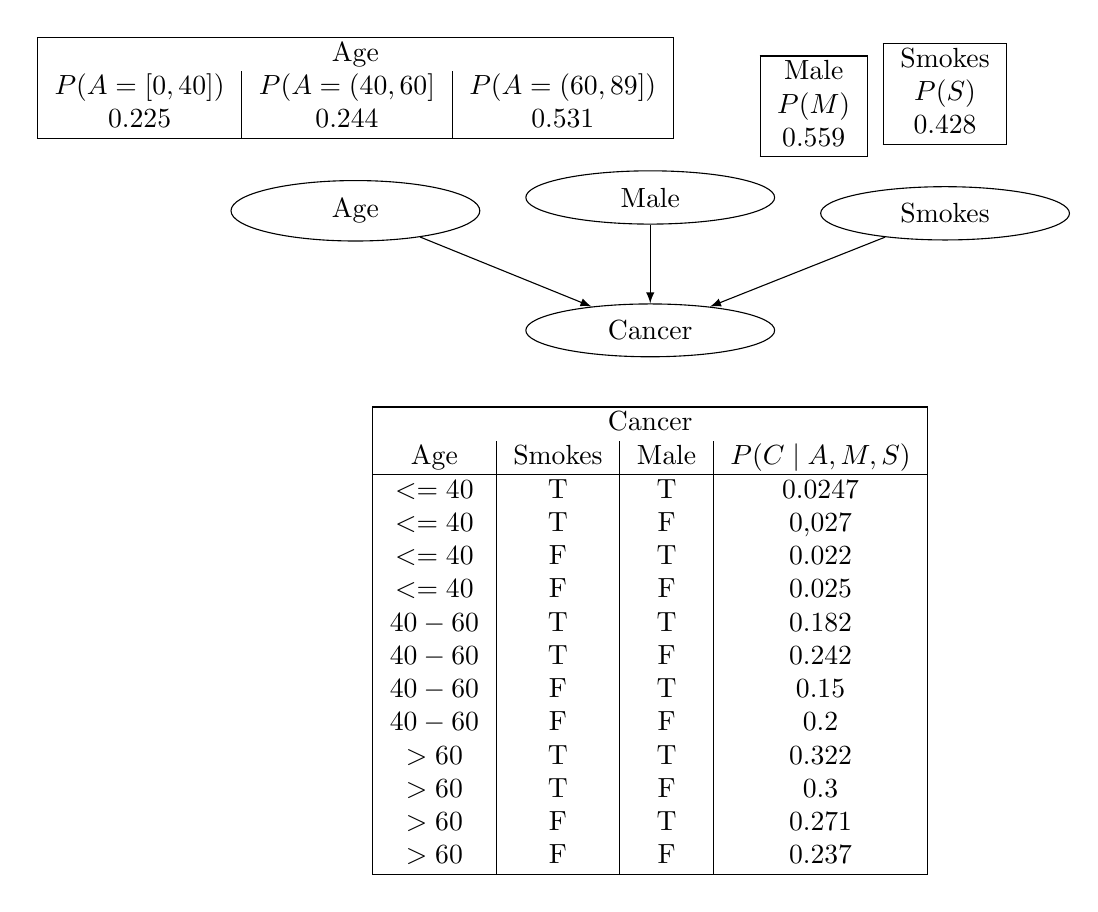
\begin{tikzpicture}[
		node distance=1cm and 1.5cm,
		mynode/.style={draw,ellipse,text width=2cm,align=center}
		]
		\node[mynode] (age) {Age};
		\node[mynode,below right=of age] (cancer) {Cancer};
		\node[mynode,above right=of cancer] (smoke) {Smokes};
		\node[mynode,above = of cancer] (male) {Male};
		\path [-latex]
		(age) edge (cancer) 
		(male) edge(cancer) 
		(smoke) edge  (cancer);
		\node[above=0.4cm of age]
		{
			\begin{tabular}{|c|c|c|}
				\hline
				\multicolumn{3}{|c|}{Age} \\
				$P(A=[0,40])$ & $P(A=(40,60]$ & $P(A=(60,89])$ \\
				$0.225$ &  $0.244$ & $0.531$ \\
				\hline
			\end{tabular}
		};
		\node[above=0.4cm of smoke]
		{
			\begin{tabular}{|c|}
				\hline
				Smokes \\
				$P(S)$ \\
				$0.428$ \\
				\hline
			\end{tabular}
		};
		\node[above right=0.2cm of male]
		{
			\begin{tabular}{|c|}
				\hline
				Male \\
				$P(M)$  \\
				$0.559$ \\
				\hline
			\end{tabular}
		};\textbf{}
		\node[below=0.5cm of cancer]
		{
			\begin{tabular}{|c|c|c|c|}
				\hline
				\multicolumn{4}{|c|}{Cancer} \\
				Age &Smokes &Male & $P(C \mid A,M,S)$  \\
				\hline
				$<=40$ & T & T & 0.0247 \\ % 58
				$<=40$ & T & F & 0,027 \\% 57
				$<=40$ & F & T & 0.022 \\% 142
				$<=40$ & F & F & 0.025 \\% 136  
				$40 - 60$ & T & T & 0.182 \\%  637
				$40 - 60$ & T & F & 0.242 \\% 500
				$40 - 60$ & F & T & 0.15 \\% 1012
				$40 - 60$ & F & F & 0.2 \\% 888
				$>60$ & T & T & 0.322 \\%2058
				$>60$ & T & F & 0.3 \\%1400
				$>60$ & F & T & 0.271\\% 3714
				$>60$ & F & F  & 0.237 \\% 2941 ACHTUNG BEI JEDEM NOCH DIVERSE DABEI
				\hline
			\end{tabular}
		};
	\end{tikzpicture}
%	\caption{MIMIC III Bayes-netz}
%\end{figure}\todo{Errors von bayes netz fixxen und Werte neu berechnen}
Das Bayes-Netz wird in ein Angreifermodell nach dem Schema aus \ref{2.2} übertragen und als beliefProgram.pbl gespeichert. Für das Alter werden dabei die \textit{annotated disjunction} verwendet, da  \\ \\
Die initStatements werden nach dem Schema von \ref{2.2} initialisiert, indem die Tabellen jeweils ein Knoten aus dem Bayes-Netz darstellen. Die Benutzer und die Sicherheitsregeln für Krebs können hierbei beliebig erstellt werden, sollten jedoch nicht zu hoch sein, da sonst die Laufzeit ungeeignet für eine Implementierung ist. \\ 
Für das füllen der Tabellen werden die \textit{HADM\_ID}s verwendet. Dafür wurde ein Bash-Skript geschrieben, dass alle \textit{HADM\_ID} s aus der Datenbank mit den benötigten Werten filtert und anschließend im passendem Format speichert.
\section{eICU}
\textbf{eICU} ist eine Datenbank, die aus einer großen Anzahl von Daten aus verschiedenen Krankenhäusern der USA besteht. Dabei ist MIMIC III nicht Teil der eICU, wodurch dies ein völlig unabhängigen Datensatz darstellt. Alle Tabellen wurden so Pseudonymisiert, dass diese dem HIPAA Standard entsprechen. Dadurch kommt es auch, dass Patienten mit einem Alter über 89 in der Tabelle nicht existieren, da diese mit \enquote{>89} dargestellt werden. Die Daten stammen aus dem Jahr 2014 bis 2015 und wurden dabei zufällig aus verschiedenen Krankenhäusern der USA gewählt und anschließend wurde jedem Krankenhausaufenthalt und Patient eine eindeutige Identifikationsnummer zugeordnet. \\ 
Die Datenbank enthält 200859 Krankenhauseinweisungen für 139367 Patienten aus 208 verschiedenen Krankenhäusern. Zu den Daten gehören Virtalparameter, Messungen, Pflegepläne, Art und Schweregrad der Krankheit, Diagnoseinformationen, Behandlungsinformationen und mehr. \\ \\
Im folgenden wird für jeden Patienten in der eICU Datenbank die Information, dass dieser Krebs hat, abgesichert. Die Wahrscheinlichkeitswerte des Vorwissens vom Angreifermodell werden aus der eICU Datenbank ausgelesen und somit hat jeder Angreifer wieder ein  perfektes Vorwissen. \todo[inline, size=\tiny]{reicht wenn man schreibt perfekt?} Dabei werden die Krankenhauseinweisungen als id gewählt. \\ 
Risikofaktoren und somit Abhängigkeiten für Krebs sind in dem Fall Alter, Geschlecht und eine Chemotherapie oder andere Onkologische Maßnahmen .\cite{13,14} Um diese Daten aus der eICU Datenbank zu erhalten werden die folgenden Tabellen benötigt : 
\begin{enumerate}
	\item Die Tabelle \textit{ADMISSIONSDX} stellt für jede Station in der eine Diagnose gestellt wurde, die Diagnoseinformationen bereit. Die Tabelle enthält Informationen zu demographischen Daten, Ein- und Ausweisungszeiten und erste Einweisungsinformationen.
	\item Die Tabelle \textit{PATIENT} enthält genauere Informationen über einen Patienten.  Dabei ist jeder Patient einer eindeutigen \textit{patientUnitStayID} zugeordnet, wodurch Patienten mehrfach auftauchen können, wenn diese mehrfach Eingewiesen wurden. Dies ist immer die Ausgangstabelle, da alle Krankenhausaufenthalte betrachtet werden. Zu den Daten gehören Informationen über das Geschlecht, Alter, ethnische Zugehörigkeit und mehr.
	\item Die Tabelle \textit{diagnosis} enthält Diagnosedaten zu jedem Krankenhausaufenthalt. Diese werden im ICD9 Format gespeichert.
	\item Die Tabelle \textit{TREATMENT } enthält Behandlungsinformationen über den Krankenhausaufenthalt.
\end{enumerate} 
Die Intervalle für das Alter wurden wie bei MIMIC III gewählt und das Alter kann einfach aus der Tabelle \textit{PATIENT} aus dem Attribut \textit{age} ausgelesen werden. Somit erhält man für die Intervalle  $(0,40]$ = 23091,  $(40,60]$ = 57065 und $(60,89]$ = 120608 Patienten. Dabei wurden 95 Patienten nicht berücksichtigt, weil das Attribut \textit{age} leer war.\\ 
Nach dem selben Prinzip wie beim Alter kann auch das Geschlecht ausgelesen werden, indem das Attribut \textit{gender} aus der Tabelle \textit{PATIENT} ausgelesen wird. Somit erhält man eine Verteilung von 92303 Frauen und 108379 Männern. Hierbei sind wieder 177 nicht berücksichtigt, weil das Attribut \textit{gender} für diese leer war. \\
Ob ein Patient eine Chemotherapie oder andere Onkologische Maßnahmen hatte, lässt sich aus der Tabelle \textit{TREATMENT } auslesen, indem man nach dem Suchwort \enquote{\textit{oncology}} und  \enquote{\textit{chemotherap}}sucht. Dabei sind diese eine garantierte Aussage darüber, ob dieser Patient Krebs hat. In der eICU Datenbank gibt es 2387 Patienten, bei denen dies der Fall ist. \\ 
Um die  Krebspatienten zu erhalten, werden aus der \textit{ADMISSIONSDX} Tabelle die \textit{icd9-codes} für Krebs gefiltert. Das führt dazu, dass 8179 Krebspatienten in der Datenbank enthalten sind. 
Daraus ergibt sich folgendes Bayes-Netz:

	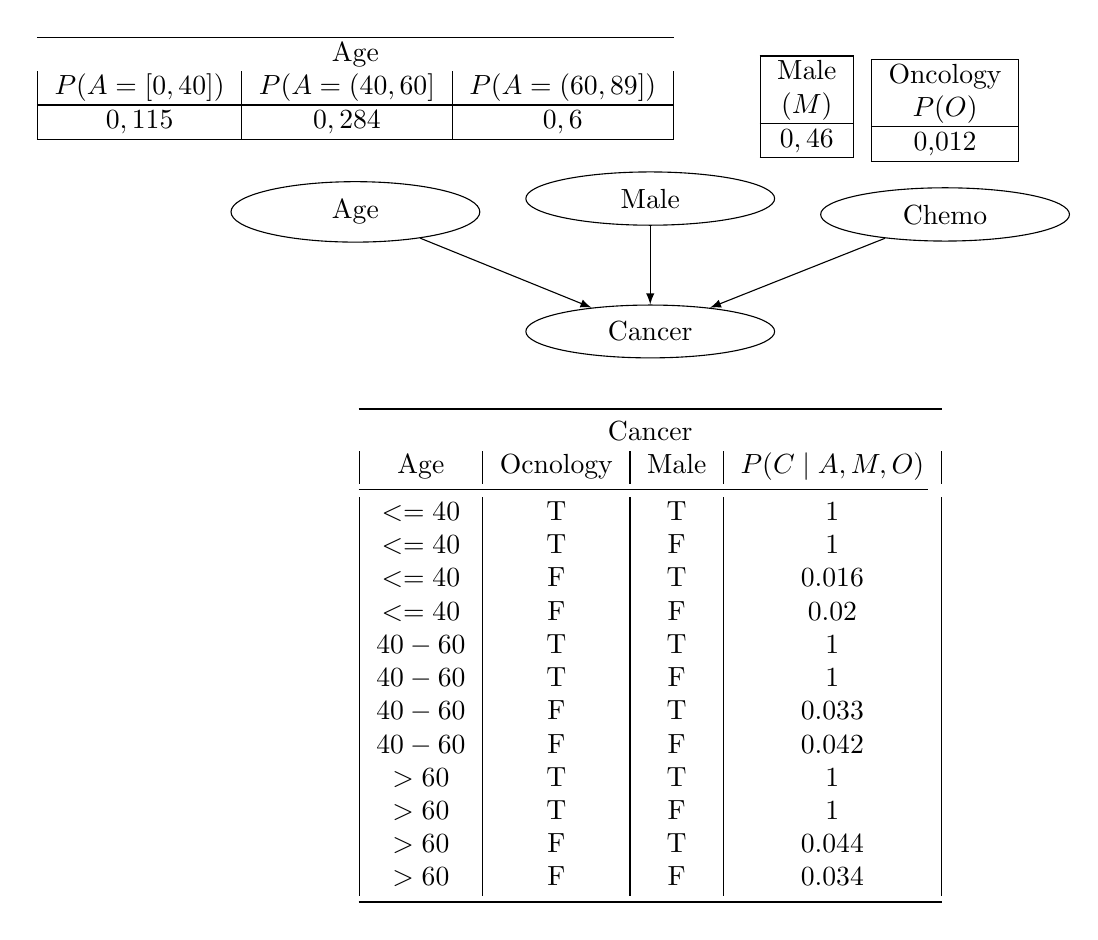
\begin{tikzpicture}[
	node distance=1cm and 1.5cm,
	mynode/.style={draw,ellipse,text width=2cm,align=center}
	]
	\node[mynode] (age) {Age};
	\node[mynode,below right=of age] (cancer) {Cancer};
	\node[mynode,above right=of cancer] (smoke) {Chemo};
	\node[mynode,above = of cancer] (male) {Male};
	\path [-latex]
	(age) edge (cancer) 
	(male) edge(cancer) 
	(smoke) edge  (cancer);
	\node[above=0.4cm of age]
	{
		\begin{tabular}{|c|c|c|}
			\hline
			\multicolumn{3}{c}{Age} \\
			$P(A=[0,40])$ & $P(A=(40,60]$ & $P(A=(60,89])$ \\
			\hline
			$0,115$ &  $0,284$ & $0,6$ \\
			\hline
		\end{tabular}
	};
	\node[above=0.2cm of smoke]
	{
		\begin{tabular}{|c|}
			\hline
			Oncology \\
			$P(O)$ \\
			\hline
			0,012 \\
			\hline
		\end{tabular}
	};
	\node[above right =0.2cm of male]
	{
		\begin{tabular}{|c|}
			\hline
			Male \\
			$(M)$ \\
			\hline
			$0,46$  \\
			\hline
		\end{tabular}
	};
	\node[below=0.5cm of cancer]
	{
		\begin{tabular}{|c|c|c|c|}
			\toprule
			\multicolumn{4}{c}{Cancer} \\
			Age &Ocnology &Male & $P(C \mid A,M,O)$  \\
			\cmidrule(r){1-4}
			$<=40$ & T & T & 1 \\
			$<=40$ & T & F & 1 \\
			$<=40$ & F & T & 0.016 \\
			$<=40$ & F & F & 0.02 \\
			$40 - 60$ & T & T & 1 \\
			$40 - 60$ & T & F & 1 \\
			$40 - 60$ & F & T & 0.033 \\
			$40 - 60$ & F & F & 0.042 \\
			$>60$ & T & T & 1 \\
			$>60$ & T & F & 1 \\
			$>60$ & F & T & 0.044\\
			$>60$ & F & F  & 0.034 \\
			\bottomrule
		\end{tabular}
	};
\end{tikzpicture}


\section{Synthea}
\textbf{Synthea} \cite{19,20} ist eine open-source Software, mit der Patientendatenbanken generiert werden können. Die demographischen Daten werden dabei anhand von öffentlich Zugänglichen demographischen Daten vom US Census Bureau \cite{21} generiert. Synthea unterstützt dabei die Generierung der Datenbank in den Formaten ccda, fhir, text und CSV. Im folgendem Fall werden ausschließlich CSV-Dateien generiert.\\  Um Synthea für Angerona kompatibel zu machen, müssen die generierten Patientenid's von UUID zu einer eindeutig identifizierbaren id, die nur aus Zahlen besteht umgewandelt werden, weil Angerona als input nur Zahlen erlaubt und die UUID noch Sonderzeichen und Buchstaben enthält. Dies kann implementiert werden, indem im Source Ordner von Synthea in der LifeCycleModule.java die Zeile 136 ersetzt wird durch folgende : 
\begin{Java}
    attributes.put(Person.ID, String.format("\%040d", new BigInteger(UUID.randomUUID().toString().replace("-", ""), 16)));
\end{Java}
Anschließend kann man mit dem Kommando \texttt{ .$\backslash$run\_synthea -p [anzahl] -o false} die CSV-Dateien generieren und in eine beliebige Datenbank übertragen. Mit -o false wird genau die Anzahl der Patienten, die übergeben werden, da sonst auch tote Patienten generiert werden würden, die Synthea Standardmäßig mitzählt.  \\ \\
Um die Daten für das Vorwissen des Angreifers zu modellieren, wird das Generic Module Framework von Synthea verwendet. Dadurch lassen sich die Abhängigkeiten für Krankheiten oder sonstige  Einweisungsgründe ablesen, indem man in der \texttt{Module Gallary} eine beliebige öffnet. Im folgenden  wird das Angreifermodell  für die Krankheit Osteoporose definiert.  \href{https://github.com/synthetichealth/synthea/wiki/Module-Gallery#Osteoporosis} 
Aus der \textit{Module Gallary} geht hervor, dass Osteoporose abhängig ist von folgenden Faktoren : 
\begin{enumerate}
	\item \textbf{Geschlecht}: Frauen haben ein erhöhtes Risiko an Osteoporose zu erkranken als Männer. Dabei haben Männer eine $0.6$ Fache geringere Wahrscheinlichkeit als Frauen.
	\item \textbf{Alter}: Personen ab 60 Jahren können erst an Osteoporose erkranken. Dabei steigt die Wahrscheinlichkeit mit dem Alter in 10er Schritten immer mehr an bis zum Alter 90, wodurch sich ein Intervall von $<60$, 60-70 , 70-80, 80-90 und $\geq 90$ ergibt.
	\item \textbf{Knochendichte(bone-density)}: Wenn die Knochendichte zwischen $-3.8$ und $-2.5$ liegt, ist dies ein garantiertes Indiz für Osteoporose.
	\item \textbf{Medikament} Bisphosphate: Wenn ein Patient das Medikament Bisphosphate verschrieben bekommen hat, dann ist dies ebenfalls ein garantiertes Indiz für Osteoporose.
\end{enumerate} 
Das Vorwissen für das Geschlecht wurde aus der demographics.csv im Synthea Verzeichniss ausgelesen, indem der durchschnitt aller Städte gebildet wurde, wobei ein Wahrscheinlichkeitswert von $0.5$ berechnet wurde. Die Daten für die Medikamente, Alter und die Knochendichte wurden aus einer Tabelle mit 100.000 Patienten gesampelt. 
\\ 
Im folgenden Bayes-Netz werden die Wahrscheinlichkeitswerte für $P(A < 60)$ nicht gelistet, weil diese die Wahrscheinlichkeit 0 haben. Ebenfalls werden die Wahrscheinlichkeiten für $P(B=TRUE)$ und $P(O=TRUE)$ nicht gelistet, weil diese die Wahrscheinlichkeit 1 haben. Dadurch ergibt sich folgendes Bayes-Netz : 

	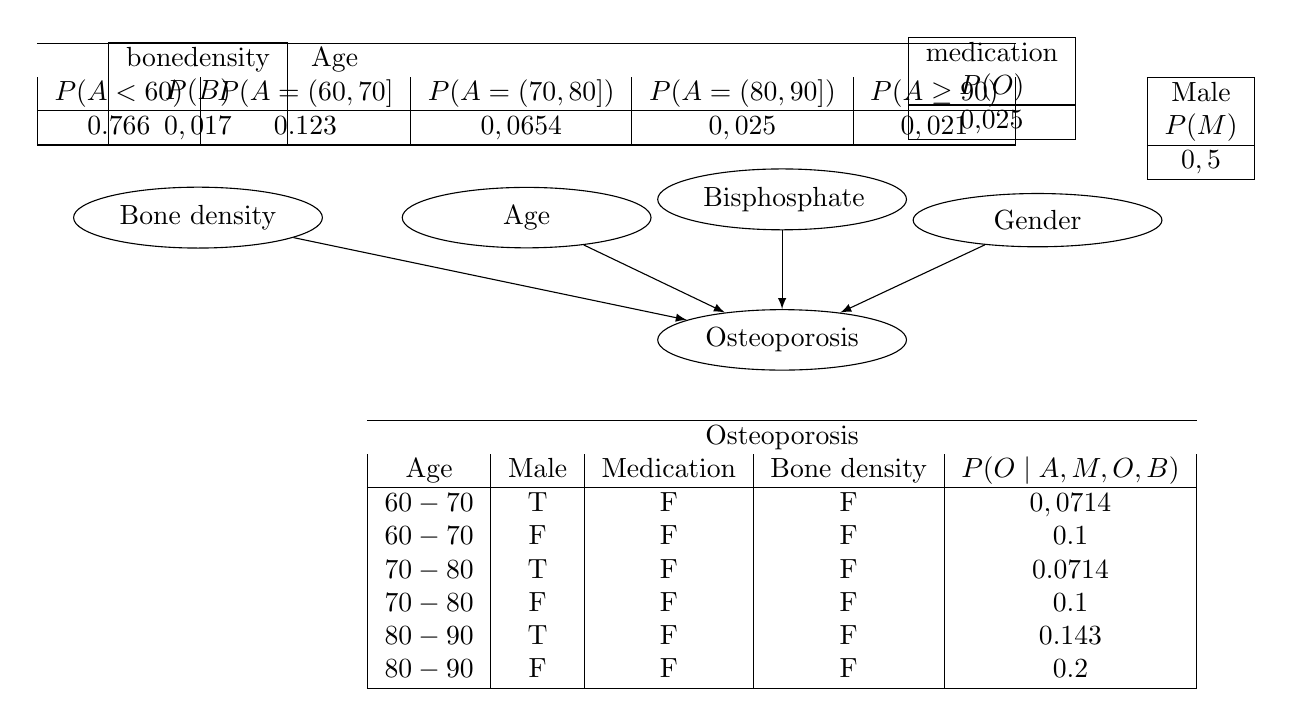
\begin{tikzpicture}[
	node distance=1cm and 1cm,
	mynode/.style={draw,ellipse,text width=2cm,align=center}
	]
	\node[mynode] (Osteoporosis) {Osteoporosis};
	\node[mynode, above left=of Osteoporosis] (age) {Age};
	\node[mynode,above right= of Osteoporosis] (Gender) {Gender};
	\node[mynode,above = of Osteoporosis] (medication) {Bisphosphate};
	\node[mynode,left = of age] (bonedensity) {Bone density};
		\path [-latex]
		(age) edge (Osteoporosis)
		(medication) edge (Osteoporosis)
		(Gender) edge(Osteoporosis)
		(bonedensity) edge(Osteoporosis);
		\node[above=0.4cm of bonedensity]
		{
			\begin{tabular}{|c|}
				\hline
				bonedensity \\
				$P(B)$ \\
				\hline
				$0,017$ \\
				\hline
			\end{tabular}
		};
			\node[above =0.4cm of age]
	{
		\begin{tabular}{|c|c|c|c|c|}
			\hline
			\multicolumn{3}{c}{Age} \\
			$P(A < 60)$ & $P(A=(60,70]$ & $P(A=(70,80])$& $P(A=(80,90])$& $P(A \geq 90)$ \\
			\hline
			$0.766$ &$0.123$ &  $0,0654$ & $0,025$ & $0,021$ \\
			\hline
		\end{tabular}
	};
		\node[above right=0.5cm of medication]
		{
			\begin{tabular}{|c|}
				\hline
				medication \\
				$P(O)$ \\
				\hline
				0,025 \\
				\hline
			\end{tabular}
		};
		\node[above right =0.2cm of Gender]
		{
			\begin{tabular}{|c|}
				\hline
				Male \\
				$P(M)$ \\
				\hline
				$0,5$  \\
				\hline
			\end{tabular}
		};
		\node[below=0.5cm of Osteoporosis]
		{
			\begin{tabular}{|c|c|c|c|c|}
				\hline
				\multicolumn{5}{c}{Osteoporosis} \\
				Age &Male &Medication & Bone density & $P(O \mid A,M,O,B)$  \\
				\hline
			$60-70$ & T & F & F & $0,0714$ \\
			$60-70$ & F & F& F & $0.1$ \\
			$70-80$ & T & F & F & $0.0714$ \\
			$70-80$ & F & F & F &$0.1$ \\
			$80-90$ & T & F & F & $0.143$ \\
			$80-90$ & F & F & F & $0.2$ \\
				\hline
			\end{tabular}
		};
	\end{tikzpicture}
Ein erweitertes Angreifermodell mit mehr Abhängigkeiten wurde durch hinzufügen des Moduls \textit{Injury} erreicht. Hierfür wurde das Angreifermodell mit dem Vorwissen für ein Knochenbruch erweitert. Ein Knochenbruch ist dabei Abhängig von Osteoporose unnd ein Knochenbruch wird unterteilt in Armbruch, Knöchelbruch, Gelenkbruch, Rippenbruch, Schlüsselbeinbruch und gebrochene Hüfte. Jedoch lässt sich dies nicht in einem für Angerona konformen Bayes-Netz modellieren, da dadurch die Bedingung verletzt wird, dass das Bayes-Netz ein Poly-tree sein muss. Durch die genannte Modellierung würde nämlich ein Zyklus entstehen zwischen den Knoten Osteoporose \leftrightarrow Knochenbruch \leftrightarrow Art des Bruches, weil z.B. ein Armbruch abhängig ist vom Knochenbruch und von Osteoporose. \\ 
Deshalb wurde die Wahrscheinlichkeit Knochenbruch als Knoten ohne Abhängigkeit definiert und die Wahrscheinlichkeit für ein Knochenbruch aus einer generierten Patientendatenbank mit 100.000 Patienten gesampled \todo[inline, size=\tiny]{gesampled? Vielleicht umschreiben}. Die Wahrscheinlichkeiten für die einzelnen Brüche können aus der Module Gallary für \textit{Injury} ausgelesen werden. Somit ergibt sich folgendes Bayes-Netz :

%\begin{tikzpicture}[
%	node distance=1cm and 1cm,
%	mynode/.style={draw,ellipse,text width=2cm,align=center}
%	]
%	\node[mynode] (Osteoporosis) {Osteoporosis};
%	\node[mynode, above left=of Osteoporosis] (age) {Age};
%	\node[mynode,above right= of Osteoporosis] (Gender) {Gender};
%	\node[mynode,above = of Osteoporosis] (medication) {Bisphosphate};
%	\node[mynode,left = of age] (bonedensity) {Bone density ($0.017$);
%%
%	\node[mynode,left = of Osteoporosis] (brokenbone) {Broken bone (14,061)};
%	\node[mynode, below right = of Osteoporosis] (brokenhip) {Broken hip};
%	\node[mynode, below = of brokenhip] (brokenclavicle) {Broken clavicle};
%	\node[mynode, left = of brokenclavicle] (brokenrib) {Broken rib};
%	\node[mynode, left = of brokenrib] (brokenwrist) {Broken wrist};
%	\node[mynode, left = of brokenwrist] (brokenankle) {Broken ankle};
%	\node[mynode, above = of brokenankle](brokenarm) {Broken arm};
%	
%	
%	
%	
%	\path [-latex]
%	(age) edge (Osteoporosis)
%	(medication) edge (Osteoporosis)
%	(Gender) edge(Osteoporosis)
%	(bonedensity) edge(Osteoporosis)
%	(Osteoporosis) edge(brokenarm)
%	(Osteoporosis) edge(brokenwrist)
%	(Osteoporosis) edge(brokenankle)
%	(Osteoporosis) edge(brokenrib)
%	(Osteoporosis) edge(brokenclavicle)
%	(Osteoporosis) edge(brokenhip)
%	(brokenbone) edge(brokenarm)
%	(brokenbone) edge(brokenwrist)
%	(brokenbone) edge(brokenankle)
%	(brokenbone) edge(brokenrib)
%	(brokenbone) edge(brokenclavicle)
%	(brokenbone) edge(brokenhip);
%	\node[above=0.4cm of age]
%	{
%		\begin{tabular}{|c|c|c|c|c|}
%			\hline
%			\multicolumn{5}{c}{Age} \\
%			$P(A < 60)$ & $P(A=[60,70))$ & $P(A=[70,80))$ & $P(A=[80,90))$& $P(A \geq 90)$  \\
%			\hline
%			$0.766$ &$0.123$ &  $0,0654$ & $0,025$ & $0,021$ \\
%			\hline
%		\end{tabular}
%	};
%	\node[above=3.4cm of medication]
%	{
%		\begin{tabular}{|c|}
%			\hline
%			Bisphosphate \\
%			$P(B)$} \\
%			\hline
%			$0.025$ \\ % 2462/99998 => 100.000 gesampled und 2462 haben das medikament verschrieben bekommen
%			\hline
%		\end{tabular}
%	};
%	\node[above=0.4cm of Gender]
%	{
%		\begin{tabular}{|c|}
%			\hline
%			Gender \\
%			$P(M)$ \\
%			\hline
%			$0,5$ \\
%			\hline
%		\end{tabular}
%	};
%	\node[above=0.4cm of Gender]
%	{
%		\begin{tabular}{|c|}
%			\hline
%			Gender \\
%			$P(M)$ \\
%			\hline
%			$0,5$ \\
%			\hline
%		\end{tabular}
%	};
%	\node[above=0.4cm of brokenarm]
%	{
%		\begin{tabular}{|c|c|c|}
%			\hline
%			\multicolumn{3}{c}{broken arm} \\
%			$BB$ & $O$ & $P(BA \mid BB,O)$  \\
%			\hline
%			T & T & $0.417$ \\
%			T & F & $0.225$ \\
%			F & T & $0$ \\
%			F & F & $0$ \\
%			\hline
%		\end{tabular}
%	};
%	\node[below=0.4cm of brokenankle]
%	{
%		\begin{tabular}{|c|c|c|}
%			\hline
%			\multicolumn{3}{c}{broken ankle} \\
%			$BB$ & $O$ & $P(BA \mid BB,O)$  \\
%			\hline
%			T & T & $0.101$ \\
%			T & F & $0.2$ \\
%			F & T & $0$ \\
%			F & F & $0$ \\
%			\hline
%		\end{tabular}
%	};
%	\node[below=0.4cm of brokenwrist]
%	{
%		\begin{tabular}{|c|c|c|}
%			\hline
%			\multicolumn{3}{c}{broken wrist} \\
%			$BB$ & $O$ & $P(BW \mid BB,O)$  \\
%\hline
%			T & T & $0.101$ \\
%			T & F & $0.2$ \\
%			F & T & $0$ \\
%			F & F & $0$ \\
%			\hline
%		\end{tabular}
%	};
%	\node[below=0.4cm of brokenrib]
%	{
%		\begin{tabular}{|c|c|c|}
%			\hline
%			\multicolumn{3}{c}{broken rib} \\
%			$BB$ & $O$ & $P(BR \mid BB,O)$  \\
%\hline
%			T & T & $0.05$ \\
%			T & F & $0.1$ \\
%			F & T & $0$ \\
%			F & F & $0$ \\
%			\hline
%		\end{tabular}
%	};
%	\node[below=0.4cm of brokenclavicle]
%	{
%		\begin{tabular}{|c|c|c|}
%			\hline
%			\multicolumn{3}{c}{broken clavicle} \\
%			$BB$ & $O$ & $P(BC \mid BB,O)$  \\
%\hline
%			T & T & $0.101$ \\
%			T & F & $0.225$ \\
%			F & T & $0$ \\
%			F & F & $0$ \\
%			\hline
%		\end{tabular}
%	};
%	\node[above=0.4cm of brokenhip]
%	{
%		\begin{tabular}{|c|c|c|}
%			\hline
%			\multicolumn{3}{c}{broken hip} \\
%			$BB$ & $O$ & $P(BH \mid BB,O)$  \\
%\hline
%			T & T & $0.23$ \\
%			T & F & $0.05$ \\
%			F & T & $0$ \\
%			F & F & $0$ \\
%			\hline
%		\end{tabular}
%	};
%	\node[below=0.5cm of brokenarm]
%	;
%\end{tikzpicture}
\section{Angreifer modellierung}

\section{Vor und nachteile}

\chapter{Laufzeiten der Patientendatenbanken}
Um die folgenden Experimente und Auswertung zu reproduzieren, sollten erstmal die Anwendungen und Einstellungen vorgestellt werden. Der genutzte Computer hat einen AMD Ryzen 2600x Sechs-Kern Prozessor die mit 3.6GHz laufen, 16GB RAM mit 2400MHz und nutzt Windows
10 Enterprise LTSC als Betriebssystem. Das Projekt wurde jedoch aus Kompatibilitätsgründen auf einer virtuellen Maschine ausgeführt. Die VM läuft auf Oracle VM VirtualBox Version 6.1.6 und nutzt Ubuntu 20.04.1 LTS. Dabei wurden der VM Sechs von Zwölf Threads und 8GB RAM bereitgestellt. \\ \\

Alle Datenbanken laufen auf einer Virtuellen Maschine in einem PowerEdge R530 Server. Dieser Server hat zwei Intel Xeon E5-2620 v3 Prozessoren 2,4GHz mit jeweils 6 Core / 12 Threads und 64GB DDR4-SDRAM. Als Datenbanksystem wird PostgreSQL Version 9.5.24 verwendet.

\chapter{Zusammenfassung und Ausblick}

% !!!!!!!!!!!!!!!!!!!!!!!!!!!!!!!!!!
% !!! Your action is needed here !!!
% !!!!!!!!!!!!!!!!!!!!!!!!!!!!!!!!!!
%
% Replace the following with your conclusion
% Ausblick : Gruppensystem einführen vlt. Vlt ist es jetzt schon möglich?, damit nicht jeder einzelnd deklariert werden muss weil sonst sau voll , 2. Nachteil : nur Numbers/integers erlaubt und z.B. standard uuid ist ein mix aus Buchstaben , Nummern und -(Sonderzeichen)


This template document got much longer than I had initially intended
with more and more hints and comments becoming part of the text. The
reason is, of course, that writing a thesis is not easy since there
are a \emph{lot} of things to consider. However, you have six months
to write your thesis, so you stand a decent chance to get most things 
right.

Do some great scientific research now and report on it in a thesis
that is a pleasure to read. 


\listoftodos



% Normally, the bibliography comes next at this point. Do *not* (try
% to) include further indices and tables like an index or
% a list of figures or a list of tables or such things. Nobody
% actually uses them and they just use up space. 
%
% You *can* however include a glossary, if this seems appropriate. It
% goes here as an unnumbered chapter. Most thesis will *not* need a
% glossary: a well-written text (re)explains strange words and
% concepts as necessary. However, there are situations where a
% glossary may be helpful.














%%%
% 
% Bibliographies
%
%%%
%
% The uzl-thesis class will load biblatex for the bibliography
% management. This is a powerful package, see its documentation for
% details. The styles will be setup correctly and automatically by
% choosing one of the two style keys as described earlier.
%
% In order for the bibliography to work, run latex in the following
% order (which is the standard order):
% 
% > lualatex thesis-example
% > bibtex thesis-example
% > lualatex thesis-example
% 
% Add BibTeX files using \addbibresource or use the {bibtex entries}
% environment (see below).
%
%%%
%
% Although everyting is normally setup automatically, you can change
% the options passed to biblatex using the key 'biblatex';
% for instance,
%
%   \UzLThesisSetup{biblatex={firstinits=false}}
%
% will switch off shortened first names. Normally, you will not need
% this key in your preamble. 
% 
% Note that the bibtex program is used as the 'backend' of biblatex
% by default (rather than biber, which is the preferred program of
% biblatex). This means that you can (and must) run *bibtex* after you
% have run lualatex on your thesis. If you wish to use biber instead
% of bibtex, say 'biblatex={backend=biber}'. 
% 
%%%
%
% The following environment is optional. It allows you to keep the
% bibtex entries for your thesis right here in the thesis file. What
% happens is that each time this tex file is processed, the contents
% of the following environment gets written to the file
% \jobname-bibtex-entries.bib (this file gets overwritten each
% time). Independently, \addbibresource{\jobname-bibtex-entries.bib}
% is always called if the file \jobname-bibtex-entries.bib
% exists. 
%
% In result, you can edit and keep the bibliography's bibtex entries
% right here. If you change something here, run latex, then bibtex,
% then latex once more.
%
% If you would like to manage the bibtex entries in a separate file,
% remove the below environment, delete the \jobname-bibtex-entries.bib
% file and instead write
%
% \addbibresource{filename-of-your-bibtex-file.bib}
%
% in the preamble.
%
%%%


% !!!!!!!!!!!!!!!!!!!!!!!!!!!!!!!!!!
% !!! Your action is needed here !!!
% !!!!!!!!!!!!!!!!!!!!!!!!!!!!!!!!!!
%
% Replace following example entries with the ones of your thesis.



% If you need to have an appendix (I advise against it), insert it
% here using, first, \appendix and then \chapter and then,
% possibly, \section. 
%
% \appendix
%
% \chapter{Technical Appendix}
%
% \section{Experimental Parameters} % possibly
%
% Again, I advise against using an appendix.


\end{document}

%  LocalWords:  LaTeX tex moretexcs Lübeck pdf uzl lualatex bibtex th
%  LocalWords:  TechReport Kernighan Lamport's Tantau's Tantau cls kZ
%  LocalWords:  Mustermann emacs oldschool pdflatex texmf utf biber
%  LocalWords:  biblatex Alphabetische Bibliographie Numerische VIIa
%  LocalWords:  varioref german Einleitung Beiträge dieser Arbeit xml
%  LocalWords:  Ergebnisse Verwandte Arbeiten Aufbau nucleotide VIIc
%  LocalWords:  ensembl amino phylogenetic Alexa Siri decrypt versa
%  LocalWords:  cryptographic pre nondeterministic deterministically
%  LocalWords:  Beutelspacher Untersuchungen zum genetischen sep llcc
%  LocalWords:  Beispiel tikz jpg png Alegrya Kasimir Malewitsch PGF
%  LocalWords:  Lamport Institut für Theoretische Informatik zu url
%  LocalWords:  Universität Springer DowneyF Downey Parameterized doi
%  LocalWords:  BibLaTeX Kime Philipp urldate Mittelbach hyperref Lua
%  LocalWords:  Rahtz Oberdiek Heiko Braams Bezos López fontspec Das
%  LocalWords:  Arseneau amsmath ist Tipps und zur Formulierung
%  LocalWords:  mathematischer Gedanken Mathematik Studienanfänger
%  LocalWords:  Albrecht Vieweg Teubner Verlag
